%! Author = rickr
%! Date = 11/27/2021
\subsection{TSP to Hamiltonian Circuit}
Consider an instance of the Traveling Salesman problem for the graph $G = (V,E)$ as shown in Figure \ref{fig:tsp}.
Each edge $uv$ has a weight $W_{uv}$ associated with it. 
\begin{figure}[h]
	\begin{center}
		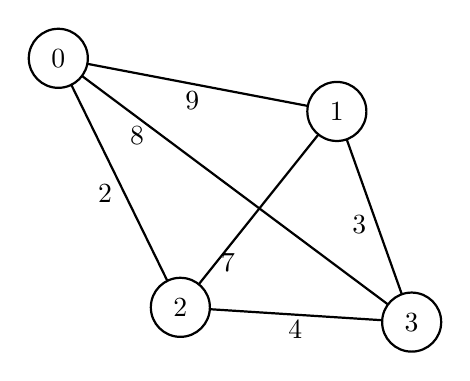
\begin{tikzpicture}[scale=0.125]
			\tikzstyle{every node}+=[inner sep=0pt]
			\draw  [thick](22,-14.2) circle (3);
			\draw  [][thick](22,-14.2) node {$0$};
			\draw  [thick](34.4,-39.5) circle (3);
			\draw  [][thick](34.4,-39.5) node {$2$};
			\draw  [thick](50.3,-19.6) circle (3);
			\draw  [][thick](50.3,-19.6) node {$1$};
			\draw  [thick](57.9,-41) circle (3);
			\draw  [][thick](57.9,-41) node {$3$};
			\draw  [][thick](23.32,-16.89) -- (33.08,-36.81);
			
			\draw [](27.5,-27.94) node [left] {$2$};
			\draw [][thick] (24.95,-14.76) -- (47.35,-19.04);
			
			\draw [](35.62,-17.49) node [below] {$9$};
			\draw [][thick] (51.3,-22.43) -- (56.9,-38.17);
			
			\draw [](53.34,-31.06) node [left] {$3$};
			\draw [][thick] (37.39,-39.69) -- (54.91,-40.81);
			
			\draw [](46.07,-40.81) node [below] {$4$};
			\draw [][thick] (24.4,-15.99) -- (55.5,-39.21);
			
			\draw [](30,-23) node [above] {$8$};
			\draw [][thick] (48.43,-21.94) -- (36.27,-37.16);
			
			\draw [](40, -35) node [left] {$7$};
		\end{tikzpicture}
		\caption{\doublespacing A graph G representing an instance of the Traveling Salesman Problem. Each node $V$ is connected via a weighted edge $E=W_{uv}$.}
		\label{fig:tsp}
	\end{center}
\end{figure}
The set of solutions to this graph can be seen in Table \ref{tab:eigenset} located in the appendix and the shortest Hamiltonian cycle that can be taken has a total distance of 18.
One possible route is $2\rightarrow3\rightarrow1\rightarrow0$. 
This route can be represented as a matrix as shown if Figure \ref{fig:matrix}, where $i$ and $p$ correspond to the city and order of traversal respectively. 
\begin{figure}[h]
	\begin{center}
		\begin{tabular}{c|cccc}
			\backslashbox{i}{p}&0 &1 &2 &3 \\
			\hline
			0& 0&0&0&1\\
			
			1& 0&0&1&0\\
			
			2& 1&0&0&0\\
			
			3& 0&1&0&0\\
		\end{tabular}
	\end{center}\caption{\doublespacing Solution to TSP in Figure \ref{fig:tsp} represented in the form of a matrix. The column $i$ represents each node, and the row $p$ corresponds to the nodes position in the traversal. A decision variable value of 1 corresponds to the path being taken.}\label{fig:matrix}
\end{figure}
The solution matrix of Figure \ref{fig:matrix} can be unpacked into the form of a vector 
\begin{equation}
	\vec{x} = \langle x_1, x_2, \dots, x_{N^2} \rangle
	\label{eq:vector}
\end{equation}
such that $x_j = x_{N \cdot i+p}$ where $N$ is the number of nodes in the graph. 
For example, the value at $x_{2,1}$ in the matrix will map to $x_9$ in the vector. Therefore, the vector representation of the solution to TSP in Figure \ref{fig:tsp} is $\vec{x} = <0,0,0,1,0,0,1,0,1,0,0,0,0,1,0,0>$. 
Applying the cost function to the eigenvector will result in an eigenvalue (the total distance traveled) of $C(\vec{x}) = 18$.

For nodes forming a traversal such that $x_{i,p}$ and $x_{i,p+1}$ are both equal to one but not connected in $G$, i.e., $(i,j)\notin E$, then an energy penalty should be imposed in the form $\sum_{i,j \notin E}\sum_p x_{i,p}x_{i,p+1}>0$ \cite{lucas2014ising}.
However, since we are only considering fully connected graphs, this term may be omitted and the net cost of a tour can be calculated from the cost function of Equation \ref{eq:cost}.
% Cost Function
\begin{equation}
	C(X)=\sum_{i,j}w_{i,j} \sum_p x_{i,p}x_{j,p+1} 
	\label{eq:cost}
\end{equation}
Where $w_{i,j}$ is the weight between nodes $i$ and $j$, and $x_{i,p}x_{j,p+1}=1$ if the route is actually taken. Inspecting the features of Figure \ref{fig:matrix}, we find that every vertex can only appear once in a cycle and each position must be occupied by a node. 
This amounts to the two constraints given in Equation \ref{eq:constraints}.
% Constraints
\begin{equation}
	\sum_p x_{i,p}=1 \quad \forall \: i \in cities \quad \text{and} \quad \sum_i x_{i,p}=1 \quad \forall \: p \in route
	\label{eq:constraints}
\end{equation}

By imposing these constraints to Equation \ref{eq:cost}, we find that the objective function to be minimized takes the form
% Distance with constraints
\begin{equation}
	C(X)=\sum_{i,j}w_{i,j} \sum_p x_{i,p}x_{j,p+1} + A\sum_p (1 - \sum_i x_{i,p})^2 + A\sum_i (1 - \sum_p x_{i,p})^2
	\label{eq:hamiltoniancircuit}
\end{equation}
where $A>W_{max}$ is a positive constant set to be much larger than maximum weight encountered during the traversal. Note that the constraints are squared so as to prevent the algorithm from diverging to negative infinity. 

To complete the preparation of TSP, we need to convert the cost function of Equation \ref{eq:cost} into a quantum Hamiltonian by changing variables from $x_i$ to the Pauli operator $\sigma_i^z$ (a $2x2$ matrix whose eigenvectors $|1,0\rangle$ and $|0,-1\rangle$ have eigenvalues (+1,-1)). 
\begin{equation}
	x_i \rightarrow \frac{ 1-\sigma_{i,p}^z}{2} \qquad \Rightarrow \qquad C(X) \rightarrow C(\sigma_{i,p}^z) \equiv H_p
	\label{eq:transformation}
\end{equation}